\documentclass[a4paper]{article}

\usepackage[T1]{fontenc}
\usepackage[italian]{babel}
\usepackage[latin1]{inputenc}
\usepackage{graphicx}
\usepackage{float}
\usepackage[margin=2 cm]{geometry}
\usepackage{multirow}
\usepackage{multicol}
\usepackage{textcomp}
\usepackage{caption}
\usepackage{amsmath}
\author{Alberto Bordin, Giulio Cappelli}
\title{Duplicatore di frequenza}
\date{14-15 Dicembre 2017}
\newcommand{\minitab}[2][l]{\begin{tabular}#1 #2\end{tabular}}


\begin{document}
	\maketitle
	
	\begin{abstract}
		 
	\end{abstract}

\section{To do}
	
\section{Teoria}

\section{Apparato sperimentale}

\section{Taratura dell'attenuatore}

\begin{multicols}{2}
	Per prima cosa abbiamo tarato l'attenuatore regolabile. Abbiamo misurato la potenza ogni 5 gradi centesimali. I dati raccolti sono riportati in appendice (Tabella \ref{tab:taratura}) e graficati in Figura \ref{fig:taratura}.
	
\subsubsection*{Discussione degli errori}
In Figura \ref{fig:taratura} abbiamo riportato errore di calibrazione, che � un errore sistematico. Nelle sezioni successive talvolta � richiesto l'uso di un errore statistico, in tal caso verr� usata la sigma relativa all'errore di digitalizzazione.

\end{multicols}

\begin{figure}[H]
	\centering
	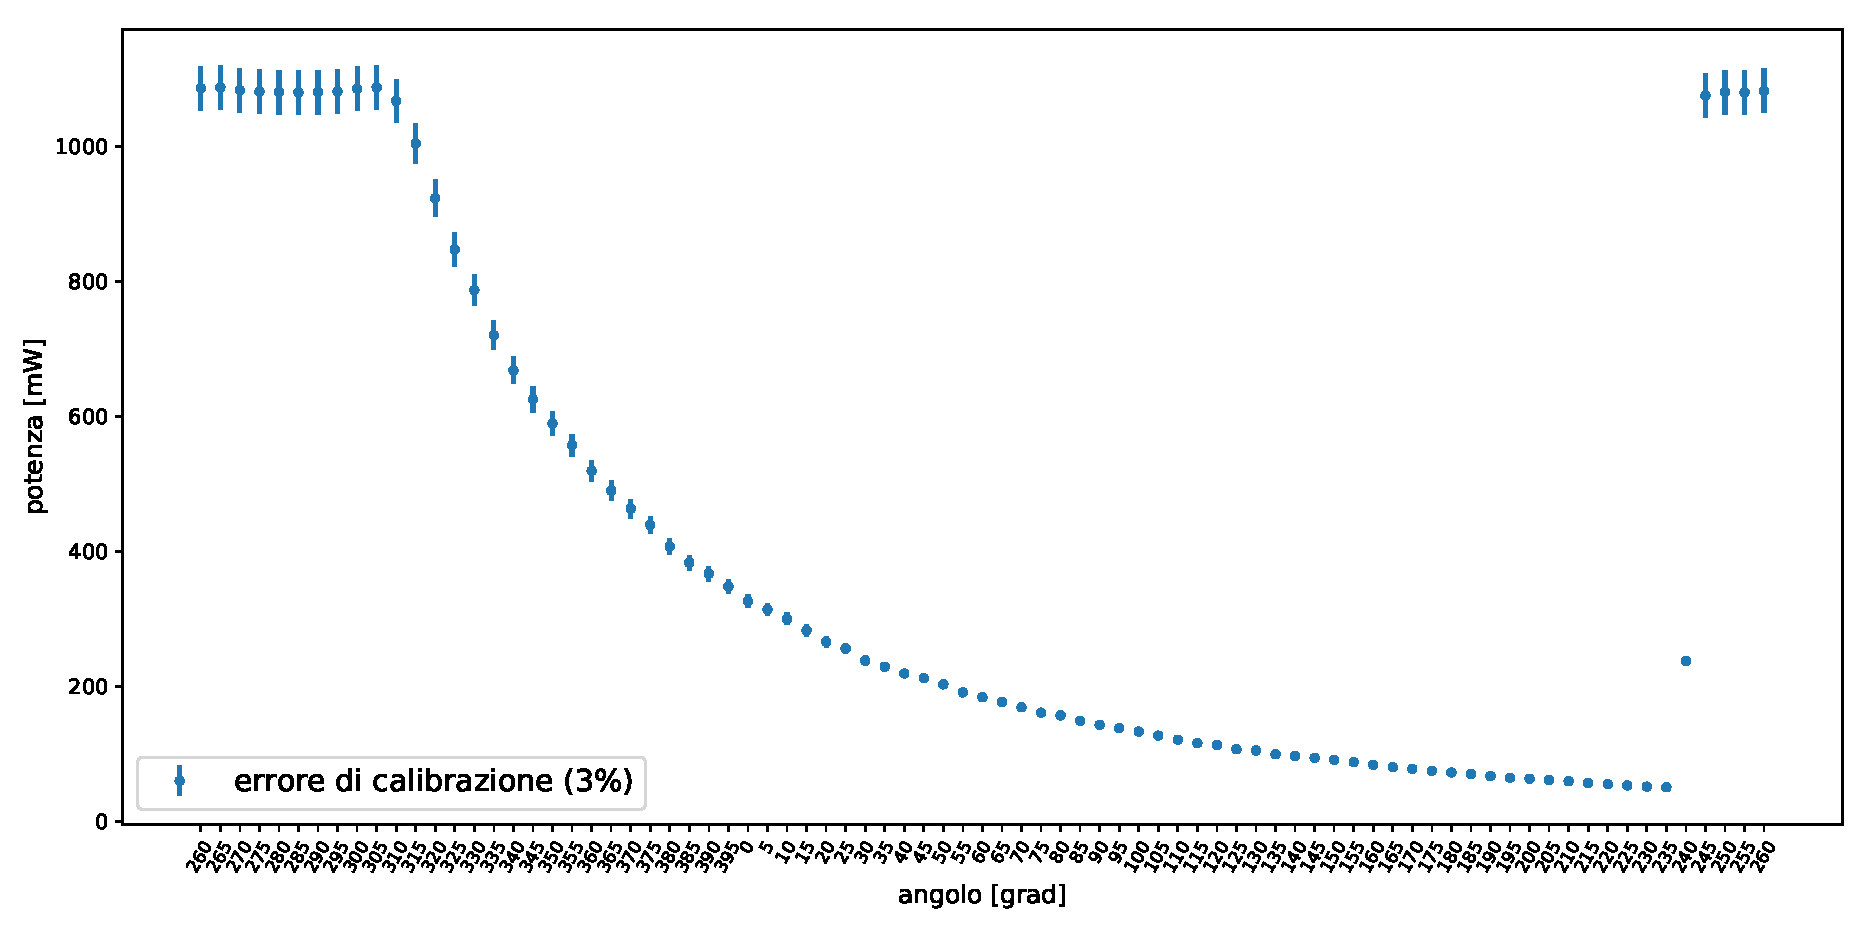
\includegraphics[width=1\textwidth]{taratura.pdf}
	\caption{Taratura dell'attenuatore regolabile.}
	\label{fig:taratura}
\end{figure}

\section{Segnale duplicato in funzione della potenza incidente}

\begin{multicols}{2}
	
\subsection{Presa dati}

Il professore ci ha rivelato che un buon segnale all'oscilloscopio � di $\sim600$ $V_{pp}$ quindi abbiamo speso le prime ore disponibili ad allineare al meglio l'apparato nella ricerca di un buon segnale, trovando al massimo $\sim400$ $V_{pp}$. Infine il professore stesso ha provato ad allineare arrivando ad un segnale di $\sim500$ $V_{pp}$. Non capiamo perch� sia stato impossibile fare di meglio.

Secondo il modello della generazione di seconda armonica con la tecnica di \textit{phase matching} conta una sola polarizzazione del laser di pompa. Il suo angolo � fissato dalla posizione dell'asse straordinario nel cristallo birifrangente, quindi l'orientazione della pompa non conta soltanto se il laser di pompa ha una polarizzazione uniforme . Nel dubbio che non fosse cos� abbiamo misurato la potenza della pompa con il \textit{power meter} frapponendo tra laser e sensore un filtro polarizzatore. In effetti abbiamo riscontrato che il laser di pompa non ha una polarizzazione uniforme: abbiamo misurato un massimo di 284.5 mW a 29� del filtro polarizzatore e un minimo di 141.5 mW a 119�. Quindi l'intensit� del segnale dipende dall'orientazione del laser di pompa. Tale fatto pu� spiegare il fatto che l'intensit� del nostro segnale non sia ottimale, tuttavia per ricavare l'angolo ottimale serve l'analisi della sezione \ref{sec:pol}. Pertanto abbiamo deciso di accontentarci di un segnale non perfetto ed evitare di ruotare il laser (e quindi di dover riallineare da capo).

Riportiamo i dati raccolti in appendice (Tabella \ref{tab:potenza}).


\subsection{Analisi dati}

	In prima analisi per verificare la legge di potenza dell'intensit� della seconda armonica abbiamo eseguito un fit con la funzione $y = ax^2$ e guardato il $\chi^2$. Ovviamente il $\chi^2$ dipende dagli errori scelti per y: l'errore di misura indicato in Tabella \ref{label} � un errore di digitalizzazione (� pari ad una tacca dell'oscilloscopio) allora per ottenere la corretta sigma da usare per il fit bisogna moltiplicarlo per $0.68 \cdot 0.5$, a questo � stato sommato in quadratura l'errore statistico della taratura dell'attenuatore (ottenuto sempre moltiplicando $0.68 \cdot 0.5$ per la sensibilit� del \textit{power meter}).
	Questa scelta d�
	\begin{align*}
	\frac{\chi^2}{dof} &= 1.27 \\
	\textrm{p-value} &= 8.2\%
	\end{align*}
	che conferma l'ipotesi di legge quadratica.
\end{multicols}
\begin{figure}[H]
	\centering
	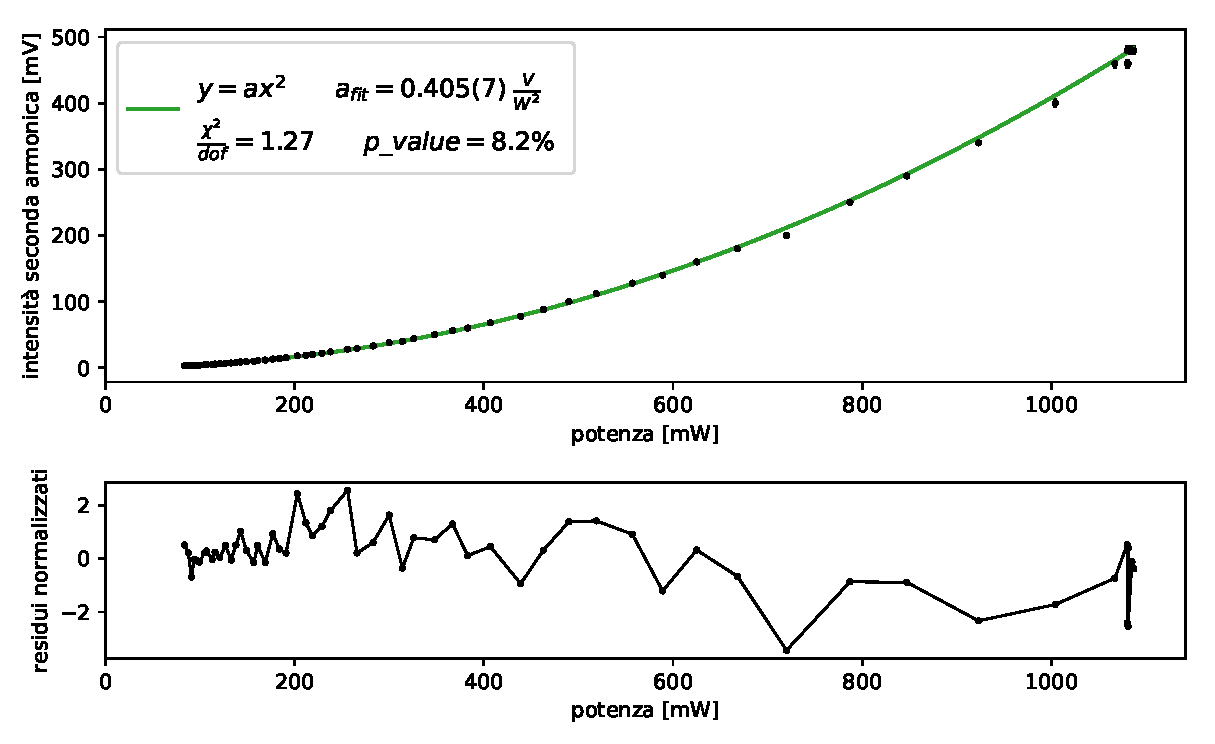
\includegraphics[width=1\textwidth]{potenza_alla2.pdf}
	\caption{Fit dell'intensit� della seconda armonica in funzione della potenza di pompa con $y = ax^2$. L'errore graficato � la somma in quadratura di errore di misura ed errore statistico della taratura.}
	\label{fig:potenza_alla2}
\end{figure}
\begin{multicols}{2}
	In seconda analisi abbiamo eseguito un fit con la funzione $y = ax^b$ (vedi Figura \ref{fig:potenza_allab}). La potenza fittata �
	\[b = 1.979(4)\]	
	
	Dal punto di vista statistico $b$ risulta incompatibile con 2 perch� l'errore dato dal fit � molto piccolo, inoltre il parametro di fit $a$ risulta incompatibile con quello risultante dal fit precedente. Tuttavia probabilmente non siamo di fronte ad una inconsistenza di risultati ma ad una sottostima degli errori. Trattare l'errore pi� accuratamente richiederebbe un analisi non banale dato che non � corretto nemmeno utilizzare l'errore di calibrazione del \textit{power meter} in quanto � errore sistematico costante.
	Pertanto ci accontentiamo del risultato trovato, che � buono all'1\%.
	
\subsection{Conclusioni}

Le misure di intensit� della seconda armonica generata in funzione della potenza di pompa sono in accordo con la legge di potenza quadratica $I_{2\omega} \propto I_{pompa}^2$. Tale risultato � stato confermato da un test del $\chi^2$ e da un fit con legge $y = ax^b$ con risultato $b = 1.98$, che 2 all'1\%.
\end{multicols}

\begin{figure}[H]
	\centering
	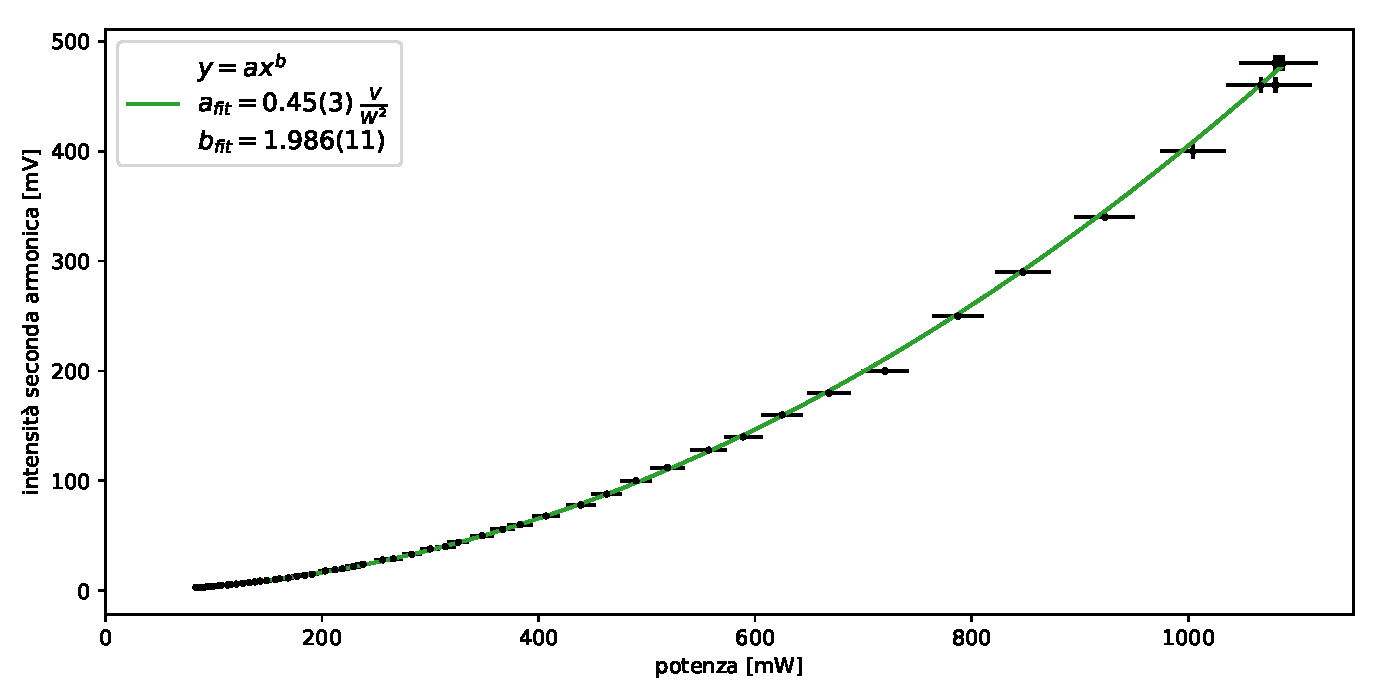
\includegraphics[width=1\textwidth]{potenza_allab.pdf}
	\caption{Fit dell'intensit� della seconda armonica in funzione della potenza di pompa con $y = ax^b$.}
	\label{fig:potenza_allab}
\end{figure}

\section{Angolo di phase-matching}

\subsection{Presa dati}

1 tabella

\subsection{Analisi dati}

1 fit a tutti a dati, 1 fit con un cut sulle code e 2 fit con gaussiana e parabola

\section{Polarizzazione}
\label{sec:pol}

\subsection{Presa dati}

\subsubsection{Polarizzazione in ingresso}

1 tabella

\subsubsection{Polarizzazione in uscita}

1 tabella

\subsection{Analisi dati}

\subsubsection{Polarizzazione in ingresso}

1 fit

\subsubsection{Polarizzazione in uscita}

1 fit

\newpage
\section*{Appendice}

\begin{table}[H]
	\centering
	\begin{tabular}{|cc|cc|cc|cc|cc|}
		\hline
		$\Theta$ [grad] & P [mW] & $\Theta$ [grad] & P [mW] & $\Theta$ [grad] & P [mW] & $\Theta$ [grad] & P [mW] & $\Theta$ [grad] & P [mW] \\
		\hline
		260 & 1086 & 345 & 625 & 30 & 238 & 115 & 116 & 200 & 63.1 \\
		265 & 1087 & 350 & 589 & 35 & 229 & 120 & 113 & 205 & 61.5 \\
		270 & 1083 & 355 & 557 & 40 & 219 & 125 & 107 & 210 & 59.5 \\
		275 & 1081 & 360 & 519 & 45 & 212 & 130 & 105 & 215 & 56.9 \\
		280 & 1080 & 365 & 490 & 50 & 203 & 135 & 99.4 & 220 & 55.1 \\
		285 & 1080 & 370 & 463 & 55 & 191 & 140 & 96.7 & 225 & 53.3 \\
		290 & 1080 & 375 & 439 & 60 & 184 & 145 & 94.0 & 230 & 51.5 \\
		295 & 1081 & 380 & 407 & 65 & 177 & 150 & 91.1 & 235 & 50.5 \\
		300 & 1085 & 385 & 383 & 70 & 169 & 155 & 87.7 & 240 & 237.4 \\
		305 & 1087 & 390 & 367 & 75 & 161 & 160 & 83.7 & 245 & 1075 \\
		310 & 1067 & 395 & 348 & 80 & 157 & 165 & 80.2 & 250 & 1080 \\
		315 & 1004 & 0 & 326 & 85 & 149 & 170 & 77.8 & 255 & 1080 \\
		320 & 923 & 5 & 314 & 90 & 143 & 175 & 74.9 & 260 & 1082 \\
		325 & 847 & 10 & 300 & 95 & 138 & 180 & 72.4 &  &  \\
		330 & 787 & 15 & 283 & 100 & 133 & 185 & 70.3 &  &  \\
		335 & 720 & 20 & 266 & 105 & 127 & 190 & 67.1 &  &  \\
		340 & 668 & 25 & 256 & 110 & 121 & 195 & 64.6 &  &  \\
		\hline
	\end{tabular}
	\caption{Taratura dell'attenuatore regolabile. Gli errori di calibrazione sulle potenze sono del 3\%. L'errore sull'angolo � inferiore a 0.5 gradi centesimali, quindi � trascurabile.}
	\label{tab:taratura}
\end{table}

\begin{table}[H]
	\centering
	\begin{tabular}{|cc|cc|cc|cc|cc|}
		\hline
		$\Theta$ [grad] & $V_{pp}$ [mV] & $\Theta$ [grad] & $V_{pp}$ [mV] & $\Theta$ [grad] & $V_{pp}$ [mV] & $\Theta$ [grad] & $V_{pp}$ [mV] & $\Theta$ [grad] & $V_{pp}$ [mV] \\
		\hline
		275&460(20)&335&200(10)&395&50(2)&55&15(1)&115&5.6(8)\\
		280&460(20)&340&180(10)&0&44(2)&60&14(1)&120&5.2(8)\\
		285&480(20)&345&160(4)&5&40(2)&65&13.2(8)&125&4.8(8)\\
		290&480(20)&350&140(4)&10&38(2)&70&11.6(8)&130&4.6(8)\\
		295&480(20)&355&128(4)&15&33(1)&75&10.8(8)&135&4.0(8)\\
		300&480(20)&360&112(4)&20&29(1)&80&10.0(8)&140&3.8(8)\\
		305&480(20)&365&100(4)&25&28(1)&85&9.2(8)&145&3.6(8)\\
		310&460(20)&370&88(4)&30&24(1)&90&8.8(8)&150&3.2(8)\\
		315&400(20)&375&78(2)&35&22(1)&95&8.0(8)&155&3.2(8)\\
		320&340(10)&380&68(2)&40&20(1)&100&7.2(8)&160&3.0(8)\\
		325&290(10)&385&60(2)&45&19(1)&105&6.8(8)& &\\
		330&250(10)&390&56(2)&50&18(1)&110&6.0(8)& &\\
		
		\hline
	\end{tabular}
	\caption{Intensit� della seconda armonica misurata con il rilevatore al silicio. Gli errori sugli angoli sono inferiori a 0.5 gradi centesimali, gli errori dell'intensit� sulle ultime cifre significative sono indicati tra parentesi.}
	\label{tab:potenza}
\end{table}



 
\end{document}